\section{Concept}
Our entire implementation is based on \cite{lafortune1993bi}. The basic idea is to shoot rays from a selected light source and the view point at the same time. All vertices of the resulting paths are connected via shadow rays (presuming that they are visible to each other) as seen in \ref{fig:shadow_rays}. The contribution to the total flux is calculated using a PDF.

\begin{figure}[htbp]
  \centering
     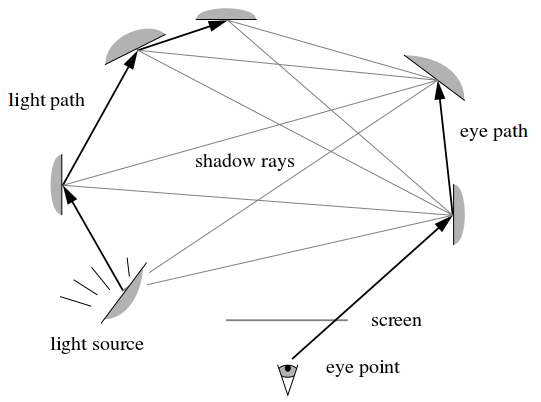
\includegraphics[width=0.8\textwidth]{pics/bi_dir_shadow_rays.png}
  \caption{Connecting light and eye paths with shadow rays \cite{lafortune1993bi}}
  \label{fig:shadow_rays}
\end{figure}